\documentclass[12pt,a4paper]{../krautsourcing/homework}
\usepackage[utf8]{inputenc}
\usepackage[ngerman]{babel}
\usepackage[T1]{fontenc}
\usepackage{amsmath}
\usepackage{graphicx}
\usepackage{amsfonts}
\usepackage{amssymb}
\usepackage{lmodern}
\usepackage{amsmath}
\usepackage{amssymb}
\usepackage{paralist}
\usepackage{tabularx}
\usepackage{tikz}
\usetikzlibrary{automata,positioning,calc}

\author{Ruben Felgenhauer,\\Alexander Hildebrandt,\\Leonhard Reichenbach}
\datef{10}{01}{2016}
%\date{\today}
\course{Formale Grundlagen der Informatik II}
\sheet{11}
\sectionprefix{Übungsaufgabe \thesheet.}
\subsectionprefix{\thesheet.}
\subsubsectioncounter{\alph{subsubsection}}
\group{06}
\subsubsectionprefix{(}
\subsubsectionsuffix{)}


%% <ltl-kram>
%% <here be dragons>
\newcommand{\tlcheckargs}[1]{
	\ifthenelse{\equal{#1}{letter}\OR\equal{#1}{symbol}}{}{%
    	\errmessage{Operator style must be either "symbol" or "letter"}
    }
}
\newcommand{\thetlstyle}{symbol}
\newcommand{\tlstyle}[1]{%
	\tlcheckargs{#1}
	\renewcommand{\thetlstyle}{#1}
}
\newcommand{\DeclareTLOperator}[3]{%
	\newcommand{#1}[1][\thetlstyle]{%
		\tlcheckargs{##1}
		\mathop{%
			\ifthenelse{\equal{#3}{}\OR\equal{##1}{letter}}{%
				\textbf{#2}
			}{%
%% </here be dragons>
%% <tweaking area>			
				\newcommand{\width}{8pt}
				\newcommand{\baseline}{-0.3pt}
				\newcommand{\preindent}{-2mu}
				\newcommand{\postindent}{-4mu}	
				\tikzset{ 
					tldrawstyle/.style={
						line width=0.5pt
					}
				}
%% </tweaking area>		
%% <here be dragons>				
				\mspace{\preindent}\raisebox{\baseline}{%
					\tikz{%
						\coordinate (bl) at (0,0);
						\coordinate (tr) at (\width,\width);
						\coordinate (tl) at (bl|-tr);
						\coordinate (br) at (tr|-bl);
						\coordinate (t)  at ($(tl)!0.5!(tr)$); 
						\coordinate (r)  at ($(tr)!0.5!(br)$);
						\coordinate (b)  at ($(bl)!0.5!(br)$);
						\coordinate (l)  at ($(tl)!0.5!(bl)$);
						\draw[tldrawstyle] #3 --cycle;
					}
				}\mspace{\postindent}
			}
		}
	}
}
\DeclareTLOperator{\tlG}{G}{%
	(tl) to[out=0,   in=180] (tr)
		 to[out=270, in=90]  (br)
		 to[out=180, in=0]   (bl)
		 to[out=90,  in=270] (tl)
}
\DeclareTLOperator{\tlF}{F}{%
	(t)  to[out=315, in=135] (r)
		 to[out=225, in=45]  (b)
		 to[out=135, in=315] (l)
		 to[out=45,  in=225] (t)
}
\DeclareTLOperator{\tlX}{X}{%
	(t)	 to[out=0,   in=90]  (r)
		 to[out=270, in=0]   (b)
		 to[out=180, in=270] (l)
		 to[out=90,  in=180] (t)
}
\DeclareTLOperator{\tlU}{U}{}
\DeclareTLOperator{\tlE}{E}{}
\DeclareTLOperator{\tlA}{A}{}
%% </here be dragons>
%% </ltl-kram>

%\newcommand{\TScell}{TS_\textit{cell}}
%\newcommand{\Mcell}{M_\textit{cell}}
\newcommand{\eLocked}{\textit{Locked}}
\newcommand{\eBattery}{\textit{Battery}}
\newcommand{\eOn}{\textit{On}}
\newcommand{\eActive}{\textit{Active}}
\newcommand{\eError}{\textit{Error}}
%\newcommand{\nmodels}{\not\models}
\newcommand{\true}{\text{True}}

\tlstyle{letter}

\begin{document}

\makeheadline

\addtocounter{section}{2}

\section{}

\subsection{}

\resizebox{\textwidth}{!}{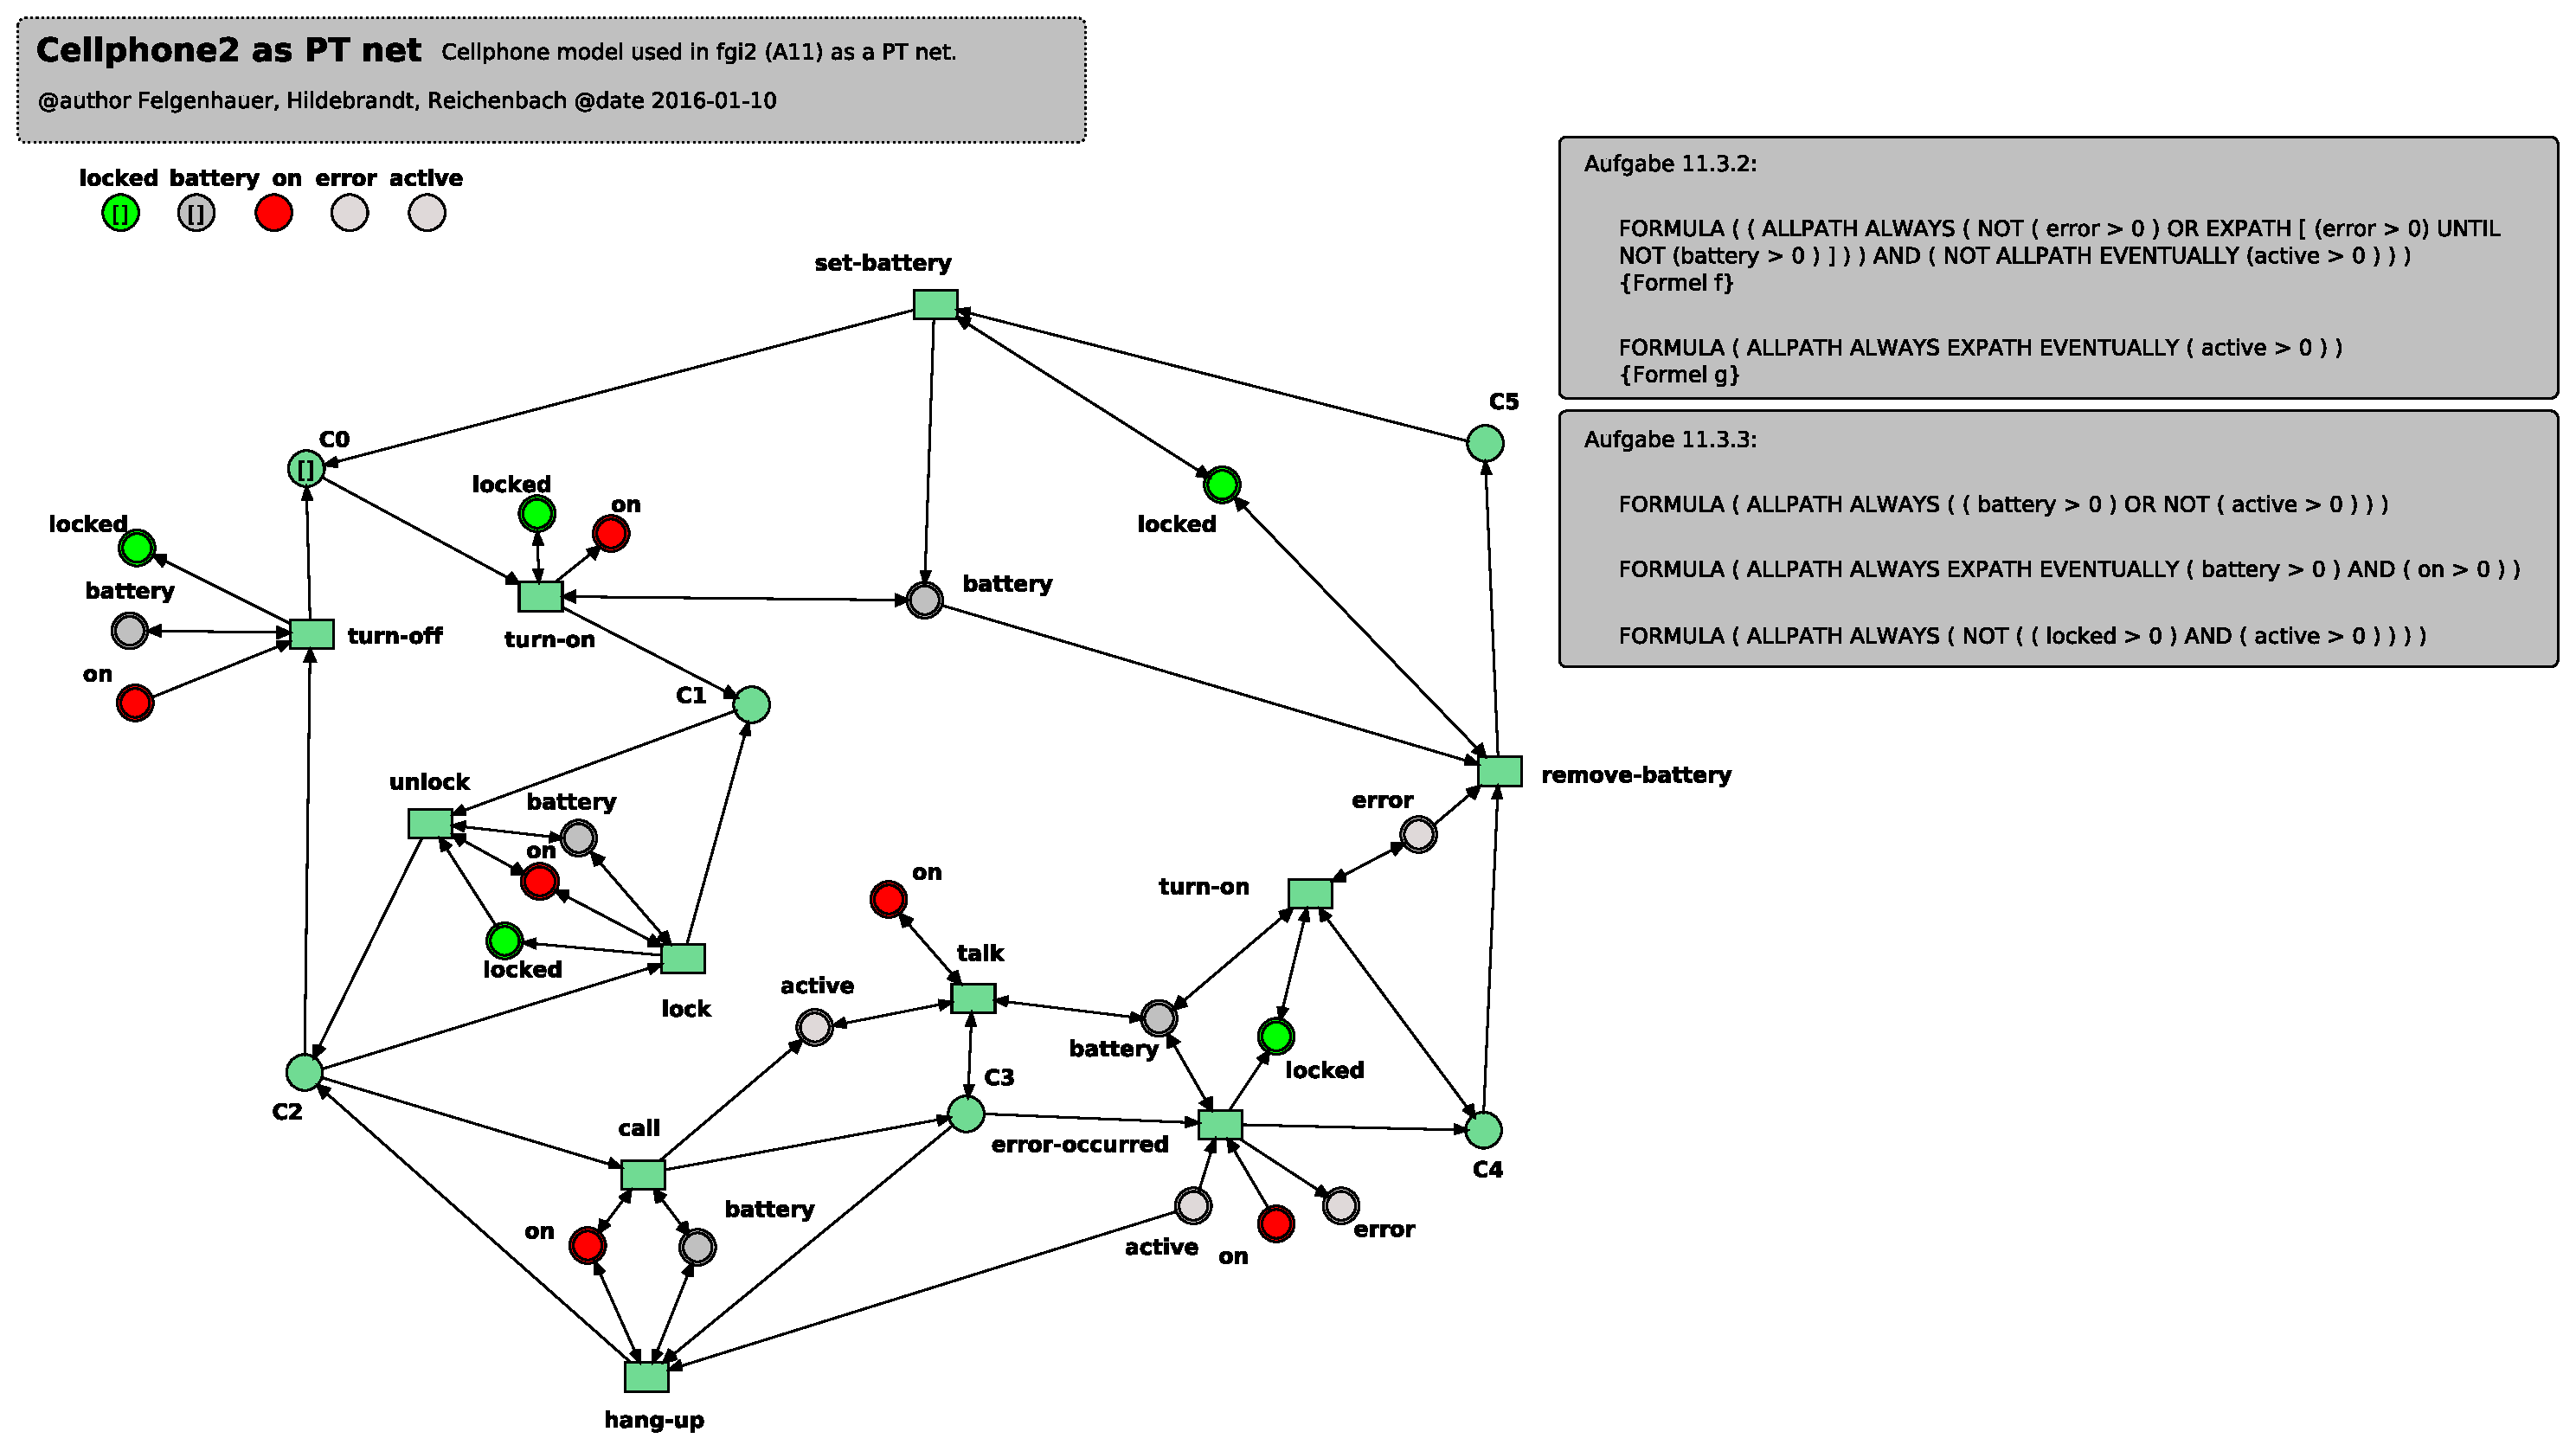
\includegraphics{cellphone.pdf}}

\subsection{}

\begin{itemize}
\item
\(\begin{aligned}
f &= \big(\tlA\tlG(\eError \Rightarrow \tlE (\eError \tlU \lnot \eBattery))\big) \land \big(\lnot \tlA \tlF \eActive \big)\\
\end{aligned}\)
\begin{verbatim}
FORMULA ( ( ALLPATH ALWAYS ( NOT ( error > 0 ) OR EXPATH [ (error > 0) UNTIL
NOT (battery > 0 ) ] ) ) AND ( NOT ALLPATH EVENTUALLY (active > 0 ) ) )
\end{verbatim}
Lola wertet die Formel zu False aus.
\item
\(\begin{aligned}
g &= \big ( \tlA \tlG \tlE \tlF (\eActive) \big )
\end{aligned}\)
\begin{verbatim}
FORMULA ( ALLPATH ALWAYS EXPATH EVENTUALLY ( active > 0 ) )
\end{verbatim}
Lola wertet die Formel zu True aus.
\end{itemize}

\newpage 
\subsection{}

\begin{itemize}
\item
\(\begin{aligned}
\tlA \tlG ( \lnot \eBattery \implies \lnot \eActive)
\end{aligned}\)
\begin{verbatim}
FORMULA ( ALLPATH ALWAYS ( ( battery > 0 ) OR NOT ( active > 0 ) ) )
\end{verbatim}
Auf allen Pfaden gilt, dass wenn keine Batterie eingelegt ist, das Telefon auch nicht aktiv ist (wahr).
\item
\(\begin{aligned}
\tlA \tlG \tlE \tlF ( \eBattery \land \eOn )
\end{aligned}\)
\begin{verbatim}
FORMULA ( ALLPATH ALWAYS EXPATH EVENTUALLY ( battery > 0 ) AND ( on > 0 ) )
\end{verbatim}
Auf allen Pfaden kommt es irgendwann wieder vor, dass sowohl eine Batterie eingelegt ist, als auch das Telefon eingeschaltet ist (wahr).
\item
\(\begin{aligned}
\tlA \tlG ( \lnot ( \eLocked \land \eActive))
\end{aligned}\)
\begin{verbatim}
FORMULA ( ALLPATH ALWAYS ( NOT ( ( locked > 0 ) AND ( active > 0 ) ) ) )
\end{verbatim}
Auf allen Pfaden gilt immer, dass das Telefon nicht gleichzeitig gesperrt und aktiv ist (wahr).
\end{itemize}

\section{}

\resizebox{\textwidth}{!}{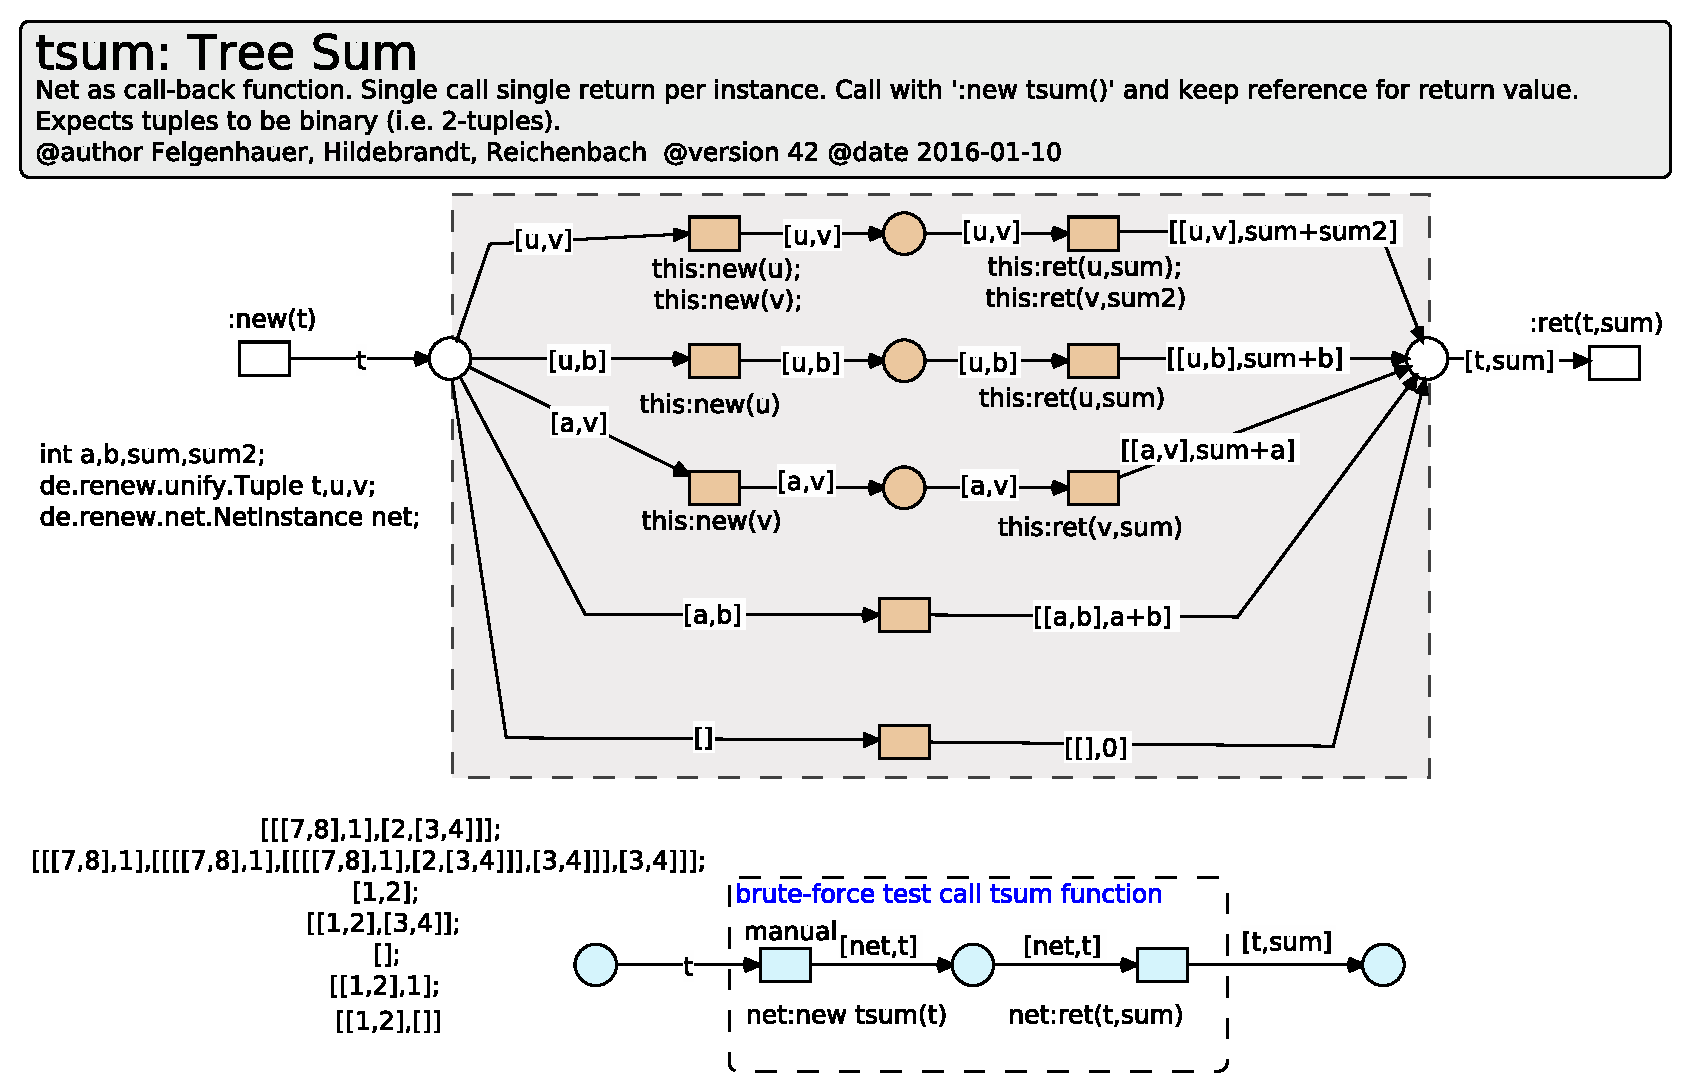
\includegraphics{tsum.pdf}}

\end{document}